\documentclass{beamer}

\usetheme{Warsaw}

\usepackage[utf8]{inputenc}
\usepackage[frenchb]{babel}
\usepackage[T1]{fontenc}

\usepackage{hyperref}

\usepackage{graphicx}

\pdfcompresslevel0

\usepackage{listings}
\usepackage{color}
\definecolor{lightgray}{rgb}{.9,.9,.9}
\definecolor{darkgray}{rgb}{.4,.4,.4}
\definecolor{purple}{rgb}{0.65, 0.12, 0.82}

\addtobeamertemplate{footline}{\hfill\insertframenumber/\inserttotalframenumber
\hspace{10em}\\}

\title{Evaluateur de $\lambda$-calcul}
\subtitle{Application web pour
  l'évaluation de $\lambda$-calcul avec représentation graphique}
\author{Vincent Botbol -- Mathieu Chailloux}

\begin{document}

\maketitle

\begin{frame}{$\lambda$-calcul -- Grammaire}
  \begin{columns}
    \begin{column}{5cm}
      \begin{itemize}
      \item $\lambda$ = ``l''
      \item arguments séparés du corps par ``.''
      \item plusieurs arguments, curryfiés plus tard
      \item application associative gauche (xxx => (x x) x)
      \end{itemize}
    \end{column}

    \begin{column}{5cm}
      \textbf{Exemples :}
      \linebreak
      \linebreak
      \textit{- lxy.y x}
      \linebreak
      \textit{- (lx.xx)(lx.xx)}
      \linebreak
      \textit{- abc}
    \end{column}

  \end{columns}

\end{frame}

\begin{frame}{$\lambda$-calcul -- Modélisation}

  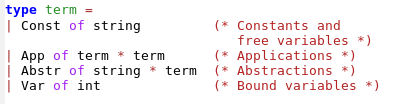
\includegraphics{lambda2.png}

\end{frame}

\begin{frame}{$\lambda$-calcul -- Indices de \emph{de Bruijn}}

  Variables liées codées par un entier.\medskip

  Valeur de cet entier = indice de l'abstraction en remontant
  l'arbre\bigskip

  \begin{columns}
    \begin{column}{5cm}
      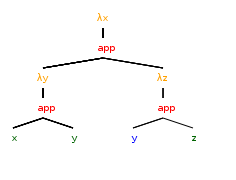
\includegraphics{lambda1.png}
    \end{column}

    \begin{column}{5cm}
      Occurences liées :
      \begin{itemize}
      \item x <=> 1
      \item y <=> 0
      \item z <=> 0
      \end{itemize}
    \end{column}
  \end{columns}

\end{frame}

\begin{frame}{$\lambda$-calcul -- $\alpha$-conversion}

  \begin{columns}
    \begin{column}{5cm}
      \begin{itemize}
      \item Changer le nom des variables liées pour éviter les ambiguïtés.
      \item Ambiguïté quand il y a 2 abstractions de même argument dans la même branche.
      \end{itemize}
    \end{column}

    \begin{column}{5cm}
      \begin{center}
        \textit{lx.(lx.x(lx.x))x}

        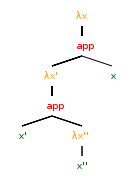
\includegraphics{lambda3.png}
      \end{center}
    \end{column}
  \end{columns}

\end{frame}

\begin{frame}{$\lambda$-calcul -- $\beta$-réduction (1)}

  Une seule règle de réduction :

  \medskip

  \textbf{($\lambda$x.M) N  -> B[N/x]}

  \medskip

  Substitution du paramètre par l'argument grâce aux indices de \textit{Bruijn}.

\end{frame}

\begin{frame}{$\lambda$-calcul -- $\beta$-réduction (2)}

    Dans la formule :
    \medskip
    \textbf{($\lambda$x.\textcolor[rgb]{1,0,0}{M}) \textcolor[rgb]{0,0,1}{N}  -> B[\textcolor[rgb]{0,0,1}{N}/x]}

    Faut-il évaluer d'abord \textcolor[rgb]{0,0,1}{N} (l'argument) ou \textcolor[rgb]{1,0,0}{M} (le corps de la fonction) ?

    \bigskip

    2 stratégies ont été implémentées :

    \begin{itemize}
    \item \textit{call-by-name} : On évalue d'abord le corps de la fonction.
    \item \textit{call-by-value} : On évalue d'abord l'argument.
    \end{itemize}

\end{frame}


\begin{frame}{Interface Graphique -- Généralités}
  \begin{itemize}
    
  \item Réalisée en \emph{OCaml} \bigskip
    
  \item \emph{Js\_of\_ocaml} : outil d'inter-opérabilité d'\emph{OCaml} vers
    \emph{JavaScript}\bigskip

  \item On accède au meilleur des deux mondes\bigskip
    %app javascript type-safe modulo la marshallisation
    
  \end{itemize}
\end{frame}

\begin{frame}{Interface Graphique -- Visualisation des $\lambda$-termes}
  \begin{itemize}
    
  \item Visualisation arborescente des termes\bigskip
    
  \item Implémentation d'un algorithme d'agencement des noeuds\bigskip

  \item On dessine dans un canvas HTML5 (grâce à
    \emph{js\_of\_ocaml})\bigskip
    
  \end{itemize}
\end{frame}

\begin{frame}{Interface Graphique -- Utilisation}
  
  \fbox{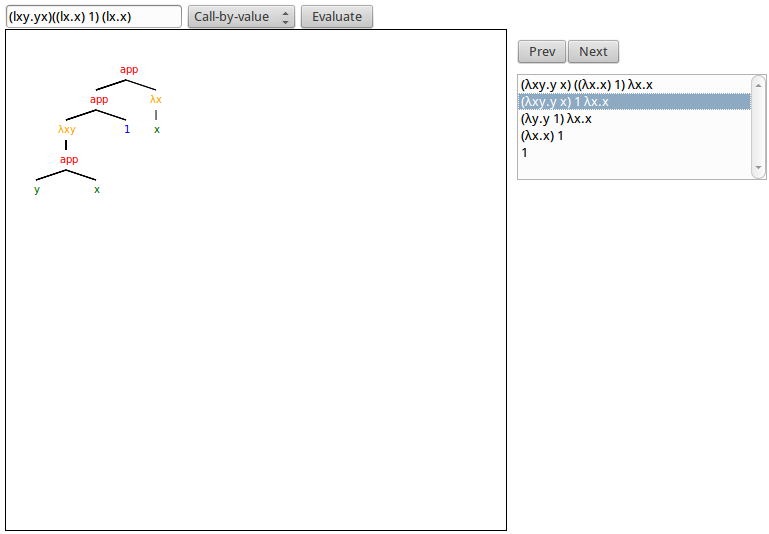
\includegraphics[scale=0.38]{screen}}
  
\end{frame}

\begin{frame}{Démonstration -- Conclusion}
  \url{http://htmlpreview.github.io/?https://github.com/vincent-botbol/lambda-eval/blob/master/index.html}
\end{frame}

\end{document}
